\documentclass[border=8pt]{standalone}
\usepackage{pgfplots}
\usepackage{xcolor}
\pgfplotsset{compat=1.18}

\definecolor{linecolor}{RGB}{52,120,190}
\definecolor{actualcolor}{RGB}{34,150,100}
\definecolor{chinchillacolor}{RGB}{190,80,50}

\begin{document}
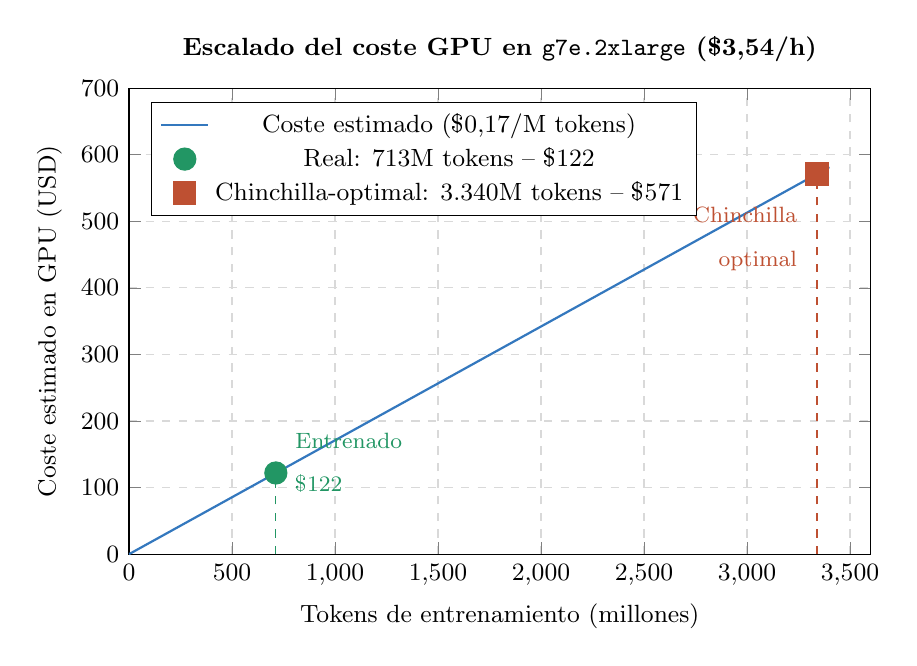
\begin{tikzpicture}
\begin{axis}[
    width=11cm,
    height=7.5cm,
    xlabel={Tokens de entrenamiento (millones)},
    ylabel={Coste estimado en GPU (USD)},
    xmin=0, xmax=3600,
    ymin=0, ymax=700,
    xtick={0,500,1000,1500,2000,2500,3000,3500},
    ytick={0,100,200,300,400,500,600,700},
    grid=major,
    grid style={dashed, gray!30},
    tick label style={font=\small},
    label style={font=\small},
    title style={font=\small\bfseries},
    title={Escalado del coste GPU en \texttt{g7e.2xlarge} (\$3,54/h)},
    legend pos=north west,
    legend style={font=\small},
]

% Linear cost curve: rate = $122 / 713M = $0.171 per million tokens
\addplot[color=linecolor, thick, domain=0:3400, samples=100] {0.171 * x};
\addlegendentry{Coste estimado (\$0,17/M tokens)}

% Actual point
\addplot[only marks, mark=*, mark size=4pt, color=actualcolor]
    coordinates {(713, 122)};
\addlegendentry{Real: 713M tokens -- \$122}

% Chinchilla point
\addplot[only marks, mark=square*, mark size=4pt, color=chinchillacolor]
    coordinates {(3340, 571)};
\addlegendentry{Chinchilla-optimal: 3.340M tokens -- \$571}

% Vertical dashed lines
\addplot[dashed, color=chinchillacolor, thin]
    coordinates {(3340,0) (3340,571)};
\addplot[dashed, color=actualcolor, thin]
    coordinates {(713,0) (713,122)};

% Annotations
\node[font=\footnotesize, color=actualcolor, anchor=west] at (axis cs:760,170) {Entrenado};
\node[font=\footnotesize, color=actualcolor, anchor=west] at (axis cs:760,105) {\$122};

\node[font=\footnotesize, color=chinchillacolor, anchor=east] at (axis cs:3290,510) {Chinchilla};
\node[font=\footnotesize, color=chinchillacolor, anchor=east] at (axis cs:3290,440) {optimal};

\end{axis}
\end{tikzpicture}
\end{document}
